\documentclass[]{article}
\usepackage{lmodern}
\usepackage{amssymb,amsmath}
\usepackage{ifxetex,ifluatex}
\usepackage{fixltx2e} % provides \textsubscript
\ifnum 0\ifxetex 1\fi\ifluatex 1\fi=0 % if pdftex
  \usepackage[T1]{fontenc}
  \usepackage[utf8]{inputenc}
\else % if luatex or xelatex
  \ifxetex
    \usepackage{mathspec}
  \else
    \usepackage{fontspec}
  \fi
  \defaultfontfeatures{Ligatures=TeX,Scale=MatchLowercase}
\fi
% use upquote if available, for straight quotes in verbatim environments
\IfFileExists{upquote.sty}{\usepackage{upquote}}{}
% use microtype if available
\IfFileExists{microtype.sty}{%
\usepackage{microtype}
\UseMicrotypeSet[protrusion]{basicmath} % disable protrusion for tt fonts
}{}
\usepackage[margin=1in]{geometry}
\usepackage{hyperref}
\hypersetup{unicode=true,
            pdftitle={Angewandte Forschungsmethodik I: Strukturgleichungsmodellierung I (SS 18)},
            pdfauthor={Übungsblatt 2: Fabio Votta, 2891518},
            pdfborder={0 0 0},
            breaklinks=true}
\urlstyle{same}  % don't use monospace font for urls
\usepackage{color}
\usepackage{fancyvrb}
\newcommand{\VerbBar}{|}
\newcommand{\VERB}{\Verb[commandchars=\\\{\}]}
\DefineVerbatimEnvironment{Highlighting}{Verbatim}{commandchars=\\\{\}}
% Add ',fontsize=\small' for more characters per line
\usepackage{framed}
\definecolor{shadecolor}{RGB}{248,248,248}
\newenvironment{Shaded}{\begin{snugshade}}{\end{snugshade}}
\newcommand{\KeywordTok}[1]{\textcolor[rgb]{0.13,0.29,0.53}{\textbf{#1}}}
\newcommand{\DataTypeTok}[1]{\textcolor[rgb]{0.13,0.29,0.53}{#1}}
\newcommand{\DecValTok}[1]{\textcolor[rgb]{0.00,0.00,0.81}{#1}}
\newcommand{\BaseNTok}[1]{\textcolor[rgb]{0.00,0.00,0.81}{#1}}
\newcommand{\FloatTok}[1]{\textcolor[rgb]{0.00,0.00,0.81}{#1}}
\newcommand{\ConstantTok}[1]{\textcolor[rgb]{0.00,0.00,0.00}{#1}}
\newcommand{\CharTok}[1]{\textcolor[rgb]{0.31,0.60,0.02}{#1}}
\newcommand{\SpecialCharTok}[1]{\textcolor[rgb]{0.00,0.00,0.00}{#1}}
\newcommand{\StringTok}[1]{\textcolor[rgb]{0.31,0.60,0.02}{#1}}
\newcommand{\VerbatimStringTok}[1]{\textcolor[rgb]{0.31,0.60,0.02}{#1}}
\newcommand{\SpecialStringTok}[1]{\textcolor[rgb]{0.31,0.60,0.02}{#1}}
\newcommand{\ImportTok}[1]{#1}
\newcommand{\CommentTok}[1]{\textcolor[rgb]{0.56,0.35,0.01}{\textit{#1}}}
\newcommand{\DocumentationTok}[1]{\textcolor[rgb]{0.56,0.35,0.01}{\textbf{\textit{#1}}}}
\newcommand{\AnnotationTok}[1]{\textcolor[rgb]{0.56,0.35,0.01}{\textbf{\textit{#1}}}}
\newcommand{\CommentVarTok}[1]{\textcolor[rgb]{0.56,0.35,0.01}{\textbf{\textit{#1}}}}
\newcommand{\OtherTok}[1]{\textcolor[rgb]{0.56,0.35,0.01}{#1}}
\newcommand{\FunctionTok}[1]{\textcolor[rgb]{0.00,0.00,0.00}{#1}}
\newcommand{\VariableTok}[1]{\textcolor[rgb]{0.00,0.00,0.00}{#1}}
\newcommand{\ControlFlowTok}[1]{\textcolor[rgb]{0.13,0.29,0.53}{\textbf{#1}}}
\newcommand{\OperatorTok}[1]{\textcolor[rgb]{0.81,0.36,0.00}{\textbf{#1}}}
\newcommand{\BuiltInTok}[1]{#1}
\newcommand{\ExtensionTok}[1]{#1}
\newcommand{\PreprocessorTok}[1]{\textcolor[rgb]{0.56,0.35,0.01}{\textit{#1}}}
\newcommand{\AttributeTok}[1]{\textcolor[rgb]{0.77,0.63,0.00}{#1}}
\newcommand{\RegionMarkerTok}[1]{#1}
\newcommand{\InformationTok}[1]{\textcolor[rgb]{0.56,0.35,0.01}{\textbf{\textit{#1}}}}
\newcommand{\WarningTok}[1]{\textcolor[rgb]{0.56,0.35,0.01}{\textbf{\textit{#1}}}}
\newcommand{\AlertTok}[1]{\textcolor[rgb]{0.94,0.16,0.16}{#1}}
\newcommand{\ErrorTok}[1]{\textcolor[rgb]{0.64,0.00,0.00}{\textbf{#1}}}
\newcommand{\NormalTok}[1]{#1}
\usepackage{longtable,booktabs}
\usepackage{graphicx,grffile}
\makeatletter
\def\maxwidth{\ifdim\Gin@nat@width>\linewidth\linewidth\else\Gin@nat@width\fi}
\def\maxheight{\ifdim\Gin@nat@height>\textheight\textheight\else\Gin@nat@height\fi}
\makeatother
% Scale images if necessary, so that they will not overflow the page
% margins by default, and it is still possible to overwrite the defaults
% using explicit options in \includegraphics[width, height, ...]{}
\setkeys{Gin}{width=\maxwidth,height=\maxheight,keepaspectratio}
\IfFileExists{parskip.sty}{%
\usepackage{parskip}
}{% else
\setlength{\parindent}{0pt}
\setlength{\parskip}{6pt plus 2pt minus 1pt}
}
\setlength{\emergencystretch}{3em}  % prevent overfull lines
\providecommand{\tightlist}{%
  \setlength{\itemsep}{0pt}\setlength{\parskip}{0pt}}
\setcounter{secnumdepth}{0}
% Redefines (sub)paragraphs to behave more like sections
\ifx\paragraph\undefined\else
\let\oldparagraph\paragraph
\renewcommand{\paragraph}[1]{\oldparagraph{#1}\mbox{}}
\fi
\ifx\subparagraph\undefined\else
\let\oldsubparagraph\subparagraph
\renewcommand{\subparagraph}[1]{\oldsubparagraph{#1}\mbox{}}
\fi

%%% Use protect on footnotes to avoid problems with footnotes in titles
\let\rmarkdownfootnote\footnote%
\def\footnote{\protect\rmarkdownfootnote}

%%% Change title format to be more compact
\usepackage{titling}

% Create subtitle command for use in maketitle
\newcommand{\subtitle}[1]{
  \posttitle{
    \begin{center}\large#1\end{center}
    }
}

\setlength{\droptitle}{-2em}
  \title{Angewandte Forschungsmethodik I: Strukturgleichungsmodellierung I (SS
18)}
  \pretitle{\vspace{\droptitle}\centering\huge}
  \posttitle{\par}
  \author{Übungsblatt 2: Fabio Votta, 2891518}
  \preauthor{\centering\large\emph}
  \postauthor{\par}
  \predate{\centering\large\emph}
  \postdate{\par}
  \date{30/04/2018}

\usepackage{pdflscape}
\usepackage{booktabs}

\begin{document}
\maketitle

\section{Recoding}\label{recoding}

\begin{Shaded}
\begin{Highlighting}[]
\NormalTok{allbus }\OperatorTok\StringTok{ }
\StringTok{  }\KeywordTok{select}\NormalTok{(}\OperatorTok{-}\NormalTok{mn11}\OperatorTok{:-}\NormalTok{mn21) }\OperatorTok\StringTok{ }\CommentTok{#select(mm05) %>% table()}
\StringTok{  }\KeywordTok{mutate}\NormalTok{(}\DataTypeTok{mm02 =} \DecValTok{8} \OperatorTok{-}\StringTok{ }\NormalTok{mm02) }\OperatorTok\StringTok{ }
\StringTok{  }\KeywordTok{mutate}\NormalTok{(}\DataTypeTok{mm05 =} \DecValTok{8} \OperatorTok{-}\StringTok{ }\NormalTok{mm05) }

\CommentTok{# allbus}
\end{Highlighting}
\end{Shaded}

\subsection{\texorpdfstring{\textbf{Beschreibung Missing
Values}}{Beschreibung Missing Values}}\label{beschreibung-missing-values}

Es zeigt sich dass nur 89 Fälle (4.3\(\%\) aller Fälle) fehlen
(Datensatz enthält nur Nicht-Muslime). Dies könnte eine unproblematische
Zahl sein, es hängt allerdings ganz davon ab ob der Mechanismus der
fehlenden Werte missing completely at random (MCAR), missing at random
(MAR) oder missing not at random (MNAR) sind. Die ersten beiden Fälle
sind eher unproblematisch, da die fehlenden Werte keinen Bias in die
Daten einführen bzw. durch beobachtete Werte entzerrt werden können.
MNAR Werte müssten allerdings als non-ignorable gewertet werden.

\begin{center}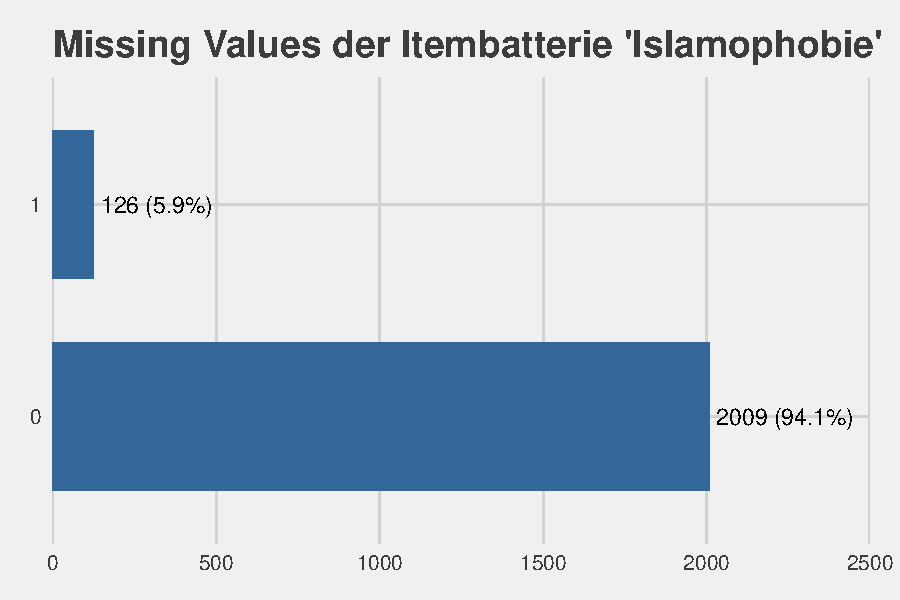
\includegraphics{ua2_files/figure-latex/unnamed-chunk-1-1} \end{center}

this could take a while

\begin{longtable}[]{@{}rrl@{}}
\caption{Little's MCAR Test}\tabularnewline
\toprule
chi2 & df & p\_value\tabularnewline
\midrule
\endfirsthead
\toprule
chi2 & df & p\_value\tabularnewline
\midrule
\endhead
332.0974 & 215 & 0.000\tabularnewline
\bottomrule
\end{longtable}

\subsection{\texorpdfstring{\textbf{Beschreibung Little's
Test}}{Beschreibung Little's Test}}\label{beschreibung-littles-test}

Der MCAR Test nach Little ist unter dem \(95\%\) Signifikanzniveau, was
bedeutet dass die fehlenden Werte als MCAR bezeichnet werden können.
Allerdings ist der Wert sehr nah an der Grenze und sollte vielleicht
doch eher mit Vorsicht gewertet werden.

\begin{table}
\begin{center}
\begin{tabular}{l c }
\hline
 & Model 1 \\
\hline
(Intercept)    & $-1.89^{***}$ \\
               & $(0.33)$      \\
Alter          & $-0.04$       \\
               & $(0.04)$      \\
isced11        & $-0.18^{**}$  \\
               & $(0.06)$      \\
Geschlecht     & $0.08$        \\
               & $(0.19)$      \\
\hline
AIC            & 940.57        \\
BIC            & 963.20        \\
Log Likelihood & -466.29       \\
Deviance       & 932.57        \\
Num. obs.      & 2116          \\
\hline
\multicolumn{2}{l}{\scriptsize{$^{***}p<0.001$, $^{**}p<0.01$, $^*p<0.05$}}
\end{tabular}
\caption{Statistical models}
\label{table:coefficients}
\end{center}
\end{table}

\begin{center}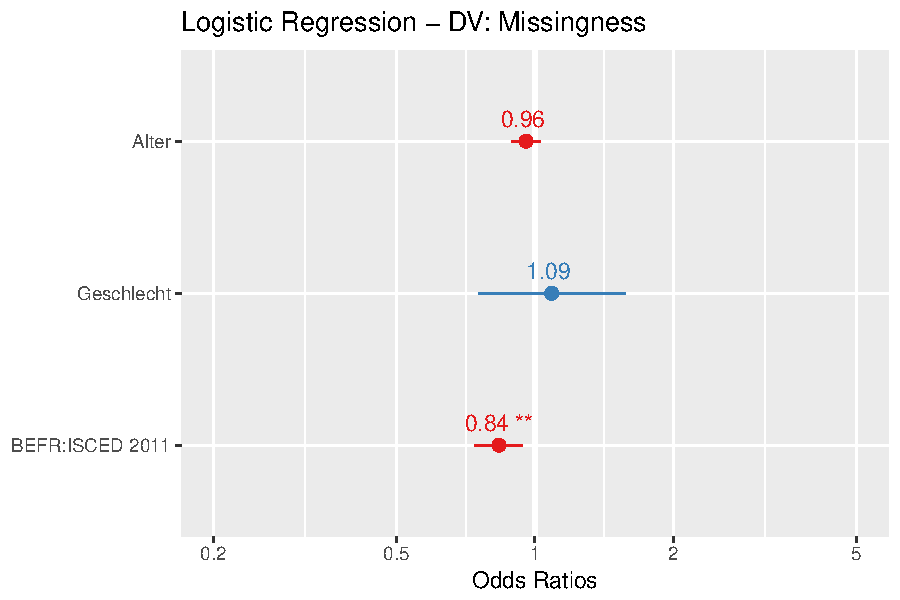
\includegraphics{ua2_files/figure-latex/unnamed-chunk-2-1} \end{center}

\begin{center}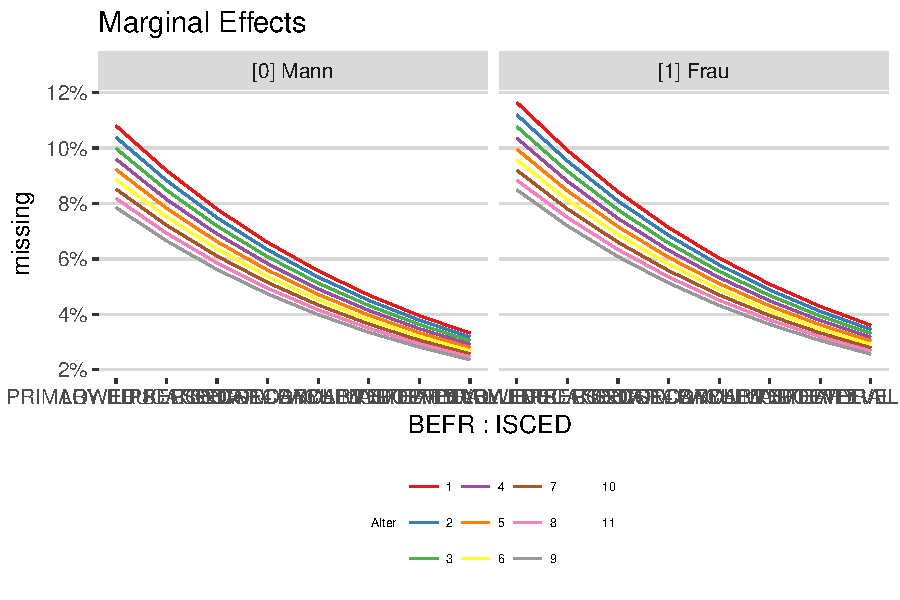
\includegraphics{ua2_files/figure-latex/unnamed-chunk-2-2} \end{center}

\subsection{\texorpdfstring{\textbf{Beschreibung Logistische
Regression}}{Beschreibung Logistische Regression}}\label{beschreibung-logistische-regression}

Die Logistische Regression mit der dichotomen abhängigen Variable
1=Fehlend und 0=Beobachtet führt zu dem Ergebnis dass keiner der
unabhängigen Variablen einen signifikanten Einfluss auf die missing
values haben. Es kann daher vorläufig davon ausgegangen werden dass die
fehlnden Werte weder auf beobachtete noch unbeobachtete Werte basieren
(und damit MCAR sind).


\end{document}
